\chapterimage{chapter-t4-bg} % Chapter heading image

\chapter{Astronomical Phenomena}

This chapter focuses on the observational side of astronomy --- what we
see when we look at the sky.

\section{The Sun}\label{the-sun}

Without a doubt, the most prominent object in the sky is the Sun. The
Sun is so bright that when it is in the sky, it's light is scattered by
the atmosphere to such an extent that almost all other objects in the
sky are rendered invisible.

The Sun is a star like many others but it is much closer to the Earth at
approximately 150 million kilometres. The next nearest star, Proxima
Centuri is approximately 260,000 times further away from us than the
Sun! The Sun is also known as \emph{Sol}, it's Latin name.

Over the course of a year, the Sun appears to move round the celestial
sphere in a great circle known as the \emph{ecliptic}. Stellarium can
draw the ecliptic on the sky. To toggle drawing of the ecliptic, press
the 4 or , key.

\emph{WARNING: Looking at the Sun can permanently damage the eye. Never
look at the Sun without using the proper filters! By far the safest way
to observe the Sun it to look at it on a computer screen, courtesy of
Stellarium!}

\section{Stars}\label{stars}

The Sun is just one of billions of stars. Even though many stars have a
much greater absolute magnitude than the Sun (the give out more light),
they have an enormously smaller apparent magnitude due to their large
distance. Stars have a variety of forms --- different sizes,
brightnesses, temperatures, and colours. Measuring the position,
distance and attributes of the stars is known as \emph{astrometry}, and
is a major part of observational astronomy.

\subsection{Multiple Star Systems}\label{multiple-star-systems}

Many stars have a stellar companions. As many as six stars can be found
orbiting one-another in close association. Such associations are known a
\emph{multiple star systems} --- \emph{binary systems} being the most
common with two stars. Multiple star systems are more common than
solitary stars, putting our Sun in the minority group.

Sometimes multiple stars orbit one-another in a way that means one will
periodically eclipse the other. These \emph{eclipsing binaries} or
\emph{Algol variables}.

\subsection{Optical Doubles \& Optical Multiples}\label{optical-doubles-optical-multiples}

Sometimes two or more stars appear to be very close to one another in
the sky, but in fact have great separation, being aligned from the point
of view of the observer but of different distances. Such pairings are
known as \emph{optical doubles} and \emph{optical multiples}.

\subsection{Constellations}\label{constellations}

The constellations are groupings of stars that are visually close to one
another in the sky. The actual groupings are fairly arbitrary ---
different cultures have group stars together into different
constellations. In many cultures, the various constellations have been
associated with mythological entities. As such people have often
projected pictures into the skies as can be seen in figure
{[}fig:ursamajor{]} which shows the constellation of Ursa Major. On the
left is a picture with the image of the mythical Great Bear, on the
right only a line-art version is shown. The seven bright stars of Ursa
Major are widely recognised, known variously as ``the plough'', the
``pan-handle'', and the ``big dipper''. This sub-grouping is known as an
\emph{asterism} --- a distinct grouping of stars. On the right, the
picture of the bear has been removed and only a constellation diagram
remains.

\begin{figure}[h]
\centering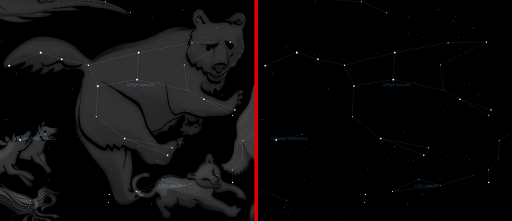
\includegraphics[scale=0.8]{uma}
%\caption{Figure caption}
\end{figure}

Stellarium can draw both constellation diagrams and artistic
representations of the constellations. Multiple sky cultures are
supported: Western, Polynesian, Egyptian and Chinese constellations are
available, although at time of writing the non-Western constellations
are not complete, and as yet there are no artistic representations of
these sky-cultures.

Aside from historical and mythological value, to the modern astronomer
the constellations provide a way to segment the sky for the purposes of
describing locations of objects, indeed one of the first tasks for an
amateur observer is \emph{learning the constellations} --- the process
of becoming familiar with the relative positions of the constellations,
at what time of year a constellation is visible, and in which
constellations observationally interesting objects reside.
Internationally, astronomers have adopted the Western (Greek/Roman)
constellations as a common system for segmenting the sky. As such some
formalisation has been adopted, each constellation having a \emph{proper
name}, which is in Latin, and a three letter abbreviation of that name.
For example, Ursa Major has the abbreviation UMa.

\subsection{Star Names}\label{star-names}

Stars can have many names. The brighter stars often have \emph{common
names} relating to mythical characters from the various traditions. For
example the brightest star in the sky, Sirius is also known as The Dog
Star (the name Canis Major --- the constellation Sirius is found in ---
is Latin for ``The Great Dog'').

There are several more formal naming conventions that are in common use.

\subsubsection{Bayer Designation}
\label{sec:concept:Bayer}
\index{Bayer}

German astronomer \emph{Johann Bayer} devised one such system in the
16-17th century. His scheme names the stars according to the
constellation in which they lie prefixed by a lower case Greek letter,
starting at $\alpha$ for (usually) the brightest star in the constellation and proceeding with $\beta, \gamma, ...$ in descending order of apparent magnitude. For example,
such a \emph{Bayer Designation} for Sirius is ``$\alpha$ Canis Majoris'' (note
that the genitive form of the constellation name is used). There are
some exceptions to the descending magnitude ordering, and some multiple
stars (both real and optical) are named with a numerical superscript
after the Greek letter, e.g. $\pi$\textsuperscript{1}...
$\pi$\textsuperscript{6} Orionis.

\subsubsection{Flamsteed Designation}
\label{sec:concepts:Flamsteed}
\index{Flamsteed}

English astronomer \emph{John Flamsteed} numbered stars in each
constellation in order of increasing right ascension followed by the
form of the constellation name, for example ``61 Cygni''.

\subsubsection{Catalogues}\label{catalogues}

As described in section \href{Star_Catalogue}{star catalogue}, various
star catalogues assign numbers to stars, which are often used in
addition to other names. Stellarium gets it's star data from the
Hipparcos catalogue, and as such stars in Stellarium are generally
referred to with their Hipparcos number, e.g. ``HP 62223''. Figure
{[}fig:starnames{]} shows the information Stellarium displays when a
star is selected. At the top, the common name and Flamsteed designation
are shown, followed by the RA/Dec coordinates, apparent magnitude,
distance and Hipparcos number.

\begin{figure}[h]
\centering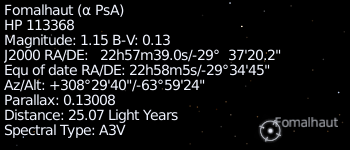
\includegraphics{names}
%\caption{Figure caption}
\end{figure}

\subsection{Spectral Type \& Luminosity
Class}\label{spectral-type-luminosity-class}

Stars have many different colours. Seen with the naked eye most appear
to be white, but this is due to the response of the eye --- at low light
levels the eye is not sensitive to colour. Typically the unaided eye can
start to see differences in colour only for stars that have apparent
magnitude brighter than 1. Betelgeuse, for example has a distinctly red
tinge to it, and Sirius appears to be blue.

By splitting the light from a star using a prism attached to a telescope
and measuring the relative intensities of the colours of light the star
emits --- the \emph{spectra} --- a great deal of interesting information
can be discovered about a star including its surface temperature, and
the presence of various elements in its atmosphere.

\begin{longtable}[c]{@{}lll@{}}
\toprule
Spectral Type & Surface Temperature ($\degree$K) & Star Colour\tabularnewline
O & 28,000---50,000 & Blue\tabularnewline
B & 10,000---28,000 & Blue-white\tabularnewline
A & 7,500---10,000 & White-blue\tabularnewline
F & 6,000---7,500 & Yellow-white\tabularnewline
G & 4,900---6,000 & Yellow\tabularnewline
K & 3,500---4,900 & Orange\tabularnewline
M & 2,000---3,500 & Red\tabularnewline
\bottomrule
\end{longtable}

Astronomers groups stars with similar spectra into \emph{spectral
types}, denoted by one of the following letters: O, B, A, F, G, K and M.
Type O stars have a high surface temperature (up to around 50,000$\degree$K)
while the at other end of the scale, the M stars are red and have a much
cooler surface temperature, typically 3000$\degree$K. The Sun is a type G star with a surface temperature of around 5,500$\degree$K. Spectral types may be further sub-divided using a numerical suffixes ranging from 0-9 where 0 is the hottest and 9 is the coolest. Table {[}fig:spectraltype{]} shows the details of the various spectral types.

For about 90\% of stars, the absolute magnitude increases as the
spectral type tends to the O (hot) end of the scale. Thus the whiter,
hotter stars tend to have a greater luminosity. These stars are called
\emph{main sequence} stars. There are however a number of stars that
have spectral type at the M end of the scale, and yet they have a high
absolute magnitude. These stars have a very large size, and consequently
are known as \emph{giants}, the largest of these known as
\emph{super-giants}.

There are also stars whose absolute magnitude is very low regardless of
the spectral class. These are known as \emph{dwarf stars}, among them
\emph{white dwarfs} and \emph{brown dwarfs}.

A \emph{luminosity class} is an indication of the type of star ---
whether it is main sequence, a giant or a dwarf. Luminosity classes are
denoted by a number in roman numerals, as described in table
{[}fig:luminosityclass{]}.

\begin{longtable}[c]{@{}ll@{}}
\toprule
\emph{Luminosity class} & \emph{Description}\tabularnewline
Ia, Ib & Super-giants\tabularnewline
II & Bright giants\tabularnewline
III & Normal giants\tabularnewline
IV & Sub-giants\tabularnewline
V & Main sequence\tabularnewline
VI & Sub-dwarfs\tabularnewline
VII & White-dwarfs\tabularnewline
\bottomrule
\end{longtable}

Plotting the luminosity of stars against their spectral type/surface
temperature, gives a diagram called a Hertzsprung-Russell diagram (after
the two astronomers \emph{Ejnar Hertzsprung} and \emph{Henry Norris
Russell} who devised it). A slight variation of this is shown in figure~\ref{fig:colourmag} (which is technically a colour/magnitude plot).

\begin{figure}[tp]
\centering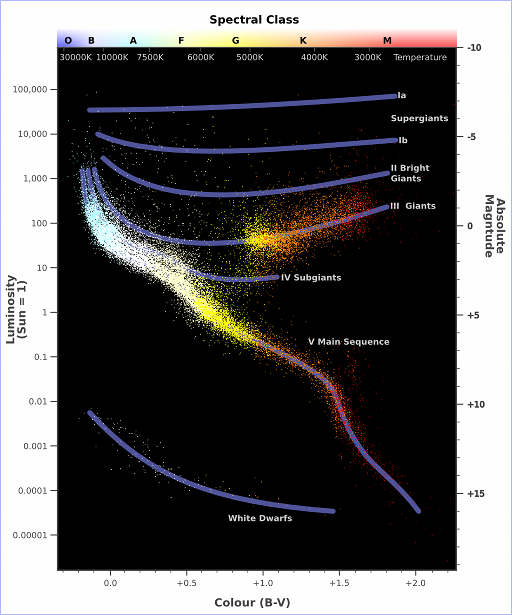
\includegraphics[width=\textwidth]{colour_magnitude_graph}
\label{fig:colourmag}
\caption{Hertzsprung-Russell Diagram}
\end{figure}

\subsection{Variables}\label{variables}

Most stars are of nearly constant luminosity. The Sun is a good example
of one which goes through relatively little variation in brightness
(usually about 0.1\% over an 11 year solar cycle). Many stars, however,
undergo significant variations in luminosity, and these are known as
\emph{variable stars}. There are many types of variable stars falling
into two categories \emph{intrinsic} and \emph{extrinsic}.

Intrinsic variables are stars which have intrinsic variations in
brightness, that is the star itself gets brighter and dimmer. There are
several types of intrinsic variables, probably the best-known and more
important of which is the Cepheid variable whose luminosity is related
to the period with which it's brightness varies. Since the luminosity
(and therefore absolute magnitude) can be calculated, Cepheid variables
may be used to determine the distance of the star when the annual
parallax is too small to be a reliable guide.

Extrinsic variables are stars of constant brightness that show changes
in brightness as seen from the Earth. These include rotating variables,
or stars whose apparent brightness change due to rotation, and eclipsing
binaries.

\section{Our Moon}\label{our-moon}

The Moon is the large satellite which orbits the Earth approximately
every 28 days. It is seen as a large bright disc in the early night sky
that rises later each day and changes shape into a crescent until it
disappears near the Sun. After this it rises during the day then gets
larger until it again becomes a large bright disc again.

\subsection{Phases of the Moon}\label{phases-of-the-moon}

As the moon moves round its orbit, the amount that is illuminated by the
sun as seen from a vantage point on Earth changes. The result of this is
that approximately once per orbit, the moon's face gradually changes
from being totally in shadow to being fully illuminated and back to
being in shadow again. This process is divided up into various phases as
described in table {[}tab:moonphases{]}.

\section{The Major Planets}\label{the-major-planets}

Unlike the stars whose relative positions remain more or less constant,
the planets seem to move across the sky over time (the word ``planet''
comes from the Greek for ``wanderer''). The planets are, like the Earth,
massive bodies that are in orbit around the Sun. Until 2006 there was no
formal definition of a planet leading to some confusion about the
classification for some bodies widely regarded as being planets, but
which didn't seem to fit with the others.

In 2006 the International Astronomical Union defined a planet as a
celestial body that, within the Solar System:

\begin{enumerate}
\item
  is in orbit around the Sun
\item
  has sufficient mass for its self-gravity to overcome rigid body forces
  so that it assumes a hydrostatic equilibrium (nearly round) shape; and
\item
  has cleared the neighbourhood around its orbit
\end{enumerate}

or within another system:

\begin{enumerate}
\item
  is in orbit around a star or stellar remnants
\item
  has a mass below the limiting mass for thermonuclear fusion of
  deuterium; and
\item
  is above the minimum mass/size requirement for planetary status in the
  Solar System.
\end{enumerate}

Moving from the Sun outwards, the major planets are: Mercury, Venus,
Earth, Mars, Jupiter, Saturn, Uranus and Neptune. Since the formal
definition of a planet in 2006 Pluto has been relegated to having the
status of \emph{dwarf planet} along with bodies such as Ceres and Eris.
See figure

\subsection{Terrestrial Planets}\label{terrestrial-planets}

The planets closest to the sun are called collectively the
\emph{terrestrial} planets. The terrestrial planets are: Mercury, Venus,
Earth and Mars.

The terrestrial planets are relatively small, comparatively dense, and
have solid rocky surface. Most of their mass is made from solid matter,
which is mostly rocky and/or metallic in nature.

\subsection{Jovian Planets}\label{jovian-planets}

Jupiter, Saturn, Uranus and Neptune make up the Jovian planets. They are
much more massive than the terrestrial planets, and do not have a solid
surface. Jupiter is the largest of all the planets with a mass over 300
times that of the Earth!

The Jovian planets do not have a solid surface - the vast majority of
their mass being in gaseous form (although they may have rocky or
metallic cores). Because of this, they have an average density which is
much less than the terrestrial planets. Saturn's mean density is only
about 0.7 g/cm\textsuperscript{3} - it would float in water!

\section{The Minor Planets}\label{the-minor-planets}

As well as the Major Planets, the solar system also contains innumerable
smaller bodies in orbit around the Sun. These are generally classed as
the \emph{minor planets}, or \emph{planetoids}, and include
\emph{asteroids}, and {[}sometimes?{]} comets.

\subsection{Asteroids}\label{asteroids}

Asteroids are celestial bodies orbiting the Sun in more or less regular
orbits mostly between Mars and Jupiter. They are generally rocky bodies
like the inner (terrestrial) planets, but of much smaller size. There
are countless in number ranging in size from about ten meters to
thousands of kilometres.

\subsection{Comets}\label{comets}

A comet is a small body in the solar system that orbits the Sun and (at
least occasionally) exhibits a coma (or atmosphere) and/or a tail.

Comets have a very eccentric orbit (very elliptical), and as such spend
most of their time a very long way from the Sun. Comets are composed of
rock, dust and ices. When they come close to the Sun, the heat
evaporates the ices, causing a gaseous release. This gas, and loose
material which comes away from the body of the comet is swept away from
the Sun by the Solar wind, forming the tail.

Comets whose orbit brings them close to the Sun more frequently than
every 200 years are considered to be \emph{short period} comets, the
most famous of which is probably Comet Halley, named after the British
astronomer Edmund Halley, which has an orbital period of roughly 76
years.

\section{Galaxies}\label{galaxies}

Stars, it seems, are gregarious - they like to live together in groups.
These groups are called galaxies. The number of stars in a typical
galaxy is literally astronomical - many \emph{billions} - sometimes ever
\emph{hundreds of billions} of stars!

Our own star, the sun, is part of a galaxy. When we look up at the night
sky, all the stars we can see are in the same galaxy. We call our own
galaxy the Milky Way (or sometimes simply ``the Galaxy'').

Other galaxies appear in the sky as dim fuzzy blobs. Only four are
normally visible to the naked eye. The Andromeda galaxy (M31) visible in
the Northern hemisphere, the two Magellanic clouds, visible in the
Southern hemisphere, and the home galaxy Milky Way, visible in parts
from north and south under dark skies.

There are thought to be billions of galaxies in the universe comprised
of an unimaginably large number of stars.

The vast majority of galaxies are so far away that they are very dim,
and cannot be seen without large telescopes, but there are dozens of
galaxies which may be observed in medium to large sized amateur
instruments. Stellarium includes images of many galaxies, including the
Andromeda galaxy (M31), the Pinwheel Galaxy (M101), the Sombrero Galaxy
(M104) and many others.

Astronomers classify galaxies according to their appearance. Some
classifications include \emph{spiral galaxies}, \emph{elliptical
galaxies}, \emph{lenticular galaxies} and \emph{irregular galaxies}.

\section{The Milky Way}\label{the-milky-way}

It's a little hard to work out what our galaxy would look like from far
away, because when we look up at the night sky, we are seeing it from
the inside. All the stars we can see are part of the Milky Way, and we
can see them in every direction. However, there is some structure. There
is a higher density of stars in particular places.

There is a band of very dense stars running right round the sky in huge
irregular stripe. Most of these stars are very dim, but the overall
effect is that on very dark clear nights we can see a large, beautiful
area of diffuse light in the sky. It is this for which we name our
galaxy.

The reason for this effect is that our galaxy is somewhat like a disc,
and we are off to one side. Thus when we look towards the centre of the
disc, we see more a great concentration of stars (there are more star in
that direction). As we look out away from the centre of the disc we see
fewer stars - we are staring out into the void between galaxies!

\section{Nebulae}\label{nebulae}

Seen with the naked eye, binoculars or a small telescope, a
\emph{nebula} (plural \emph{nebulae}) are fuzzy patches on the sky.
Historically, the term referred to any extended object, but the modern
definition excludes some types of object such as galaxies.

Observationally, nebulae are popular objects for amateur astronomers -
they exhibit complex structure, spectacular colours and a wide variety
of forms. Many nebulae are bright enough to be seen using good
binoculars or small to medium sized telescopes, and are a very
photogenic subject for astro-photographers.

Nebulae are associated with a variety of phenomena, some being clouds of
interstellar dust and gas in the process of collapsing under gravity,
some being envelopes of gas thrown off during a supernova event (so
called \emph{supernova remnants}), yet others being the remnants of
solar systems around dead stars (\emph{planetary nebulae}).

Examples of nebulae for which Stellarium has images include the Crab
Nebula (M1), which is a supernova remnant and the Dumbbell Nebula (M27)
which is a planetary nebula.

\section{Meteoroids}\label{meteoroids}

These objects are small pieces of space debris left over from the early
days of the solar system that orbit the Sun. They come in a variety of
shapes, sizes an compositions, ranging from microscopic dust particles
up to about ten meters across.

Sometimes these objects collide with the Earth. The closing speed of
these collisions is generally extremely high (tens or kilometres per
second). When such an object ploughs through the Earth's atmosphere, a
large amount of kinetic energy is converted into heat and light, and a
visible flash or streak can often be seen with the naked eye. Even the
smallest particles can cause these events which are commonly known as
\emph{shooting stars}.

While smaller objects tend to burn up in the atmosphere, larger, denser
objects can penetrate the atmosphere and strike the surface of the
planet, sometimes leaving meteor craters.

Sometimes the angle of the collision means that larger objects pass
through the atmosphere but do not strike the Earth. When this happens,
spectacular fireballs are sometimes seen.

\emph{Meteoroids} is the name given to such objects when they are
floating in space.

A \emph{Meteor} is the name given to the visible atmospheric phenomenon.

\emph{Meteorites} is the name given to objects that penetrate the
atmosphere and land on the surface.

\section{Eclipses}\label{eclipses}

Eclipses occur when an apparently large celestial body (planet, moon
etc.) moves between the observer (that's you!) and a more distant object
- the more distant object being eclipsed by the nearer one.

\subsection{Solar Eclipses}\label{solar-eclipses}

Solar eclipses occur when our Moon moves between the Earth and the Sun.
This happens when the inclined orbit of the Moon causes its path to
cross our line of sight to the Sun. In essence it is the observer
falling under the shadow of the moon.

There are three types of solar eclipses:

\textbf{Partial} The Moon only covers part of the Sun's surface.

\textbf{Total} The Moon completely obscures the Sun's surface.

\textbf{Annular} The Moon is at aphelion (furthest from Earth in its
elliptic orbit) and its disc is too small to completely cover the Sun.
In this case most of the Sun's disc is obscured - all except a thin ring
around the edge.

\subsection{Lunar Eclipses}\label{lunar-eclipses}

Lunar eclipses occur when the Earth moves between the Sun and the Moon,
and the Moon is in the Earth's shadow. They occur under the same basic
conditions as the solar eclipse but can occur more often because the
Earth's shadow is so much larger than the Moon's.

Total lunar eclipses are more noticeable than partial eclipses because
the Moon moves fully into the Earth's shadow and there is very
noticeable darkening. However, the Earth's atmosphere refracts light
(bends it) in such a way that some sunlight can still fall on the Moon's
surface even during total eclipses. In this case there is often a marked
reddening of the light as it passes through the atmosphere, and this can
make the Moon appear a deep red colour.

\section{Catalogues}\label{catalogues-1}

Astronomers have made various catalogues of objects in the heavens.
Stellarium makes use of several well known astronomical catalogues.

\subsection{Hipparcos}\label{hipparcos}

Hipparcos (for High Precision Parallax Collecting Satellite) was an
astrometry mission of the European Space Agency (ESA) dedicated to the
measurement of stellar parallax and the proper motions of stars. The
project was named in honour of the Greek astronomer Hipparchus.

Ideas for such a mission dated from 1967, with the mission accepted by
ESA in 1980. The satellite was launched by an Ariane 4 on 8 August 1989.
The original goal was to place the satellite in a geostationary orbit
above the earth, however a booster rocket failure resulted in a highly
elliptical orbit from 315 to 22,300 miles altitude. Despite this
difficulty, all of the scientific goals were accomplished.
Communications were terminated on 15 August 1993.

The program was divided in two parts: the \emph{Hipparcos experiment}
whose goal was to measure the five astrometric parameters of some
120,000 stars to a precision of some 2 to 4 milli arc-seconds and the
\emph{Tycho experiment}, whose goal was the measurement of the
astrometric and two-colour photometric properties of some 400,000
additional stars to a somewhat lower precision.

The final Hipparcos Catalogue (120,000 stars with 1 milli arc-second
level astrometry) and the final Tycho Catalogue (more than one million
stars with 20-30 milli arc-second astrometry and two-colour photometry)
were completed in August 1996. The catalogues were published by ESA in
June 1997. The Hipparcos and Tycho data have been used to create the
Millennium Star Atlas: an all-sky atlas of one million stars to visual
magnitude 11, from the Hipparcos and Tycho Catalogues and 10,000
non-stellar objects included to complement the catalogue data.

There were questions over whether Hipparcos has a systematic error of
about 1 milli arc-second in at least some parts of the sky. The value
determined by Hipparcos for the distance to the Pleiades is about 10\%
less than the value obtained by some other methods. By early 2004, the
controversy remained unresolved.

Stellarium uses the Hipparcos Catalogue for star data, as well as having
traditional names for many of the brighter stars. The stars tab of the
search window allows for searching based on a Hipparcos Catalogue number
(as well as traditional names), e.g. the star Sadalmelik in the
constellation of Aquarius can be found by searching for the name, or
it's Hipparcos number, 109074.

\subsection{The Messier Objects}\label{the-messier-objects}

The \emph{Messier} objects are a set of astronomical objects catalogued
by Charles Messier in his catalogue of \emph{Nebulae and Star Clusters}
first published in 1774. The original motivation behind the catalogue
was that Messier was a comet hunter, and was frustrated by objects which
resembled but were not comets. He therefore compiled a list of these
objects.

The first edition covered 45 objects numbered M1 to M45. The total list
consists of 110 objects, ranging from M1 to M110. The final catalogue
was published in 1781 and printed in the \emph{Connaissance des Temps}
in 1784. Many of these objects are still known by their Messier number.

Because the Messier list was compiled by astronomers in the Northern
Hemisphere, it contains only objects from the north celestial pole to a
celestial latitude of about $-35\degree$. Many impressive Southern objects, such
as the Large and Small Magellanic Clouds are excluded from the list.
Because all of the Messier objects are visible with binoculars or small
telescopes (under favourable conditions), they are popular viewing
objects for amateur astronomers. In early spring, astronomers sometimes
gather for ``Messier Marathons'', when all of the objects can be viewed
over a single night.

Stellarium includes images of many Messier objects.

\section{Observing Hints}\label{observing-hints}

When star-gazing, there's a few little things which make a lot of
difference, and are worth taking into account.

\textbf{Dark skies} For many people getting away from light pollution
isn't an easy thing. At best it means a drive away from the towns, and
for many the only chance to see a sky without significant glow from
street lighting is on vacation. If you can't get away from the cities
easily, make the most of it when you are away.

\textbf{Wrap up warm} The best observing conditions are the same
conditions that make for cold nights, even in the summer time. Observing
is not a strenuous physical activity, so you will feel the cold a lot
more than if you were walking around. Wear a lot of warm clothing, don't
sit/lie on the floor (at least use a camping mat... consider taking a
deck-chair), and take a flask of hot drink.

\textbf{Dark adaptation} The true majesty of the night sky only becomes
apparent when the eye has had time to become accustomed to the dark.
This process, known as dark adaptation, can take up to half and hour,
and as soon as the observer sees a bright light they must start the
process over. Red light doesn't compromise dark adaptation as much as
white light, so use a red torch if possible (and one that is as dim as
you can manage with). A single red LED light is ideal.

\textbf{The Moon} Unless you're particularly interested in observing the
Moon on a given night, it can be a nuisance---it can be so bright as
to make observation of dimmer objects such as nebulae impossible. When
planning what you want to observe, take the phase and position of the
Moon into account. Of course Stellarium is the ideal tool for finding
this out!

\textbf{Averted vision} A curious fact about the eye is that it is more
sensitive to dim light towards the edge of the field of view. If an
object is slightly too dim to see directly, looking slightly off to the
side but concentrating on the object's location can often reveal it.

\textbf{Angular distance} Learn how to estimate angular distances. Learn
the angular distances described in section~\ref{sec:concepts:units:angles:handyAngles}. If you
have a pair of binoculars, find out the angular distance across the
field of view and use this as a standard measure.


%%% Local Variables: 
%%% mode: latex
%%% TeX-master: "guide"
%%% End: 
